%!TEX root = /Users/jakubkonka/Thesis/Thesis.tex
\chapter{Dynamics of Network Selection in the Digital Marketplace} % (fold)
\label{cha:dynamics_of_network_selection_in_the_digital_marketplace}

\minitoc
\vspace{10mm}

The results presented in the previous chapter describe only a single stage of the selection process employed in the Digital Marketplace (DMP); i.e., a one-shot DMP auction. As such, the temporal (or dynamic) aspect of the process was neglected. The main reason for such a decision was as follows. Concentrating only on a single stage of the process considerably simplified the inherent analytical complexity of the problem and rendered the analysis tractable in case of two competing bidders. As a result, light was shed on the appropriateness of the DMP auction as a network selection mechanism at least in case of two bidders. In other words, if the results of the analysis of the one-shot DMP auction were unfavorable, then that would already render the mechanism inappropriate, and hence, little would be gained from the inclusion of the temporal aspect in the analysis.

On the other hand, it is important to consider the temporal aspect of the selection process since network selection evolves over time. For example, parameters such as reputation of each network operator, number of subscribers (and price weights), etc., which were considered static thus far, will change over time since the reputation of each network operator depends on their past (service provision) history, and more than one subscriber will enter the marketplace at any one time (and hence, price weights will vary over time).

\section{Mathematical Description} % (fold)
\label{sec:mathematical_description_dynamic}
The conceptual description of the dynamics of network selection mechanism in the DMP is as follows. The subscribers post service requests, and the network operators compete over them. The entire exchange is implemented as a procurement first-price sealed-bid (FPA) auction. The auctions operate in real time, and transaction volumes and prices reflect the relative status of supply and demand. In order to simplify the modeling, it is assumed that the probability of two auctions occurring at the same instance of time is zero. Therefore, the network operators cannot bid at two auctions simultaneously. The subscribers generate a stream of service requests, characterized by a price weight and additional attributes, according to some predetermined probability distribution function. The service request attributes are currently considered to include service type, and required bit-rate.

Since the service requests are generated over time, the network operators repeatadly compete with each other in a series of FPA auctions. Thus, from the game theoretic perspective, the network selection mechanism is akin to a repeated game where each consecutive auction constitutes a stage game~\cite{BasarOlsder1999, Gibbons92}. If we further assume that the costs of network operators may vary over time (i.e., the costs may change with each consecutive service request), then the game becomes a repeated game of incomplete information. As we will demonstrate below, the analytical analysis of this game in search of an (optimal) equilibrium bidding behavior of the network operators is intractable. Therefore, a more experimental approach will be taken; that is, the problem will be analyzed using simulation modeling approach.

In what follows, a rigorous description of the network selection process in the DMP is loosely based on the work of Figliozzi \emph{et al.}~\cite{FigliozziJaillet2008}. Although Figliozzi's work covers the dynamic analysis of a transportation marketplace, it bears many similarities to the operation of the DMP. Let $\{s_1,\ldots,s_M\}$ be the set of arriving service requests such that $s_i = (s^w_i, s^{attr}_i)$ for all $i\in I$, where $I=\{1,\ldots,M\}$ is the set of indices, $s^w_i\in [0,1]$ is the subscriber's price weight, and $s^{attr}_i\in S^{attr}$ is a $k$-tuple of attributes describing the service request. The set of all service request attribute $k$-tuples, $S^{attr}$, is left open-ended; however, at a bare minimum, it should consist of pairs ($2$-tuples) of service type and required bit-rate. For example, the web-browsing service requiring $512$ kbps bit-rate would be described by a pair $s_i^{attr} = (s_i^{type},s_i^{bw}) = (\text{``web''}, 512)$, while the email service requiring 256 kbps by a pair $(\text{``email''}, 256)$.

Let the service request/auction arrival epochs be $\{t_1,\ldots,t_M\}$ such that $t_i < t_{i+1}$ for all $i\in I$, and $t_i$ represents the arrival time of service request $s_i$ for all $i$. It is assumed that there is a one-to-one correspondence between $t_i$ and $s_i$ for all $i$. Furthermore, the service requests and their arrival times are not known in advance; i.e., they are assumed to come from some probability distribution with outcomes $\{\omega_1,\ldots,\omega_M\}$ such that $\omega_i = (t_i, s_i)$ for all $i$.

Following the notation from the previous chapters, let $N$ denote the set of network operators such that $|N| = n < \infty$; that is, there are $n$ network operators competing in the DMP. At any stage $i$, that is at an auction for service request $s_i$, each network operator $j\in N$ submits a bid $b^j_i\in\mathbb{R}_+$. It is further assumed that at each stage, every network operator must participate in an auction. Let $z^j_i\in Z$ denote the available bandwidth of network operator $j$ at time instant $i$ for all $i\in I$ and $j\in N$. Thus, the cost of servicing request $s_i$ by network operator $j$ with available bandwidth $z^j_i$ is denoted by $c^j_i = c^j_i(s_i,z^j_i)$. The cost is assumed private knowledge and, without loss of generality, it is further assumed $c^j_i\in [0,1]$ for all $i,j$.

Furthermore, at each stage $i$, each network operator $j$ is characterized by a reputation rating $r^j_i$ such that $r^j_i\in[0,1]$ for all $i,j$. As in the previous chapter, the reputation ratings are assumed common knowledge. It is further assumed they vary over time, thus reflecting the credibility of network operators in dealing with the subscribers' requests. To this end, each subscriber is assumed to have a binary perception of quality of service; that is, they may either be satisfied or dissatisfied with the service offered by a network operator. More formally, let $\sigma^j_i$ represent the satisfaction of the subscriber requesting the service $s_i$ which is handled by the network operator $j$ such that, for all $i,j$,
\begin{equation}
  \label{eq:def_users_satisfaction_dynamic}
  \sigma^j_i = \left\{
  \begin{array}{ll}
    1 &\text{if satisfied},\\
    0 &\text{otherwise}.
  \end{array}\right.
\end{equation}
It is further assumed that the subscriber is satisfied with the service if the available (at the time of service request) bandwidth of the serving network operator exceeds the required bit-rate of the service; that is,
\begin{equation}
  \label{eq:def_users_satisfaction_bandwidth_dynamic}
  \sigma^j_i = \left\{
  \begin{array}{ll}
    1 &\text{if } s_i^{bw} \le z_i^j,\\
    0 &\text{otherwise}.
  \end{array}\right.
\end{equation}
The motivation for such a simple model of the subscriber's satisfaction is as follows: since it is difficult to quantify how the subscribers perceive satisfaction with the service, rather than experimenting with probabilistic distribution of subscribers' satisfaction, we keep it simple and concentrate on more technical aspects of the DMP such as the bidding behavior of the network operators, or the reputation rating update system.

Since any one service request $i$ can be handled by a single network operator $j$, each network operator will be generating a binary sequence of user satisfaction reports over time; that is, a sequence $(\sigma^j_i)_{i\in I,j\in N}$. In turn, this sequence will then be used to compute and update the network operator's reputation rating. Currently, an adaptation of the reputation update formula proposed by Le Bodic \emph{et al.}~\cite{DMLeBodic00} is assumed; that is,
\begin{equation}
  \label{eq:def_rep_update_lebodic_dynamic}
  r^j_{i+1} = \frac{\displaystyle\sum_{k=i-(d-1)}^{i}{(1-\sigma^j_k)}}{d} \quad\text{for all }i=d,\ldots,M \text{ and }j\in N,
\end{equation}
where $d\in \mathbb{Z}_+$ is the window size. Since $\sigma^j_i$ is only defined for $i\ge 1$, it is further assumed that
\begin{equation*}
  r^j_k = 0.5 \quad\text{for all }k=1,\ldots,d-1\text{ and }j\in N.
\end{equation*}
Therefore, $r^j_k=0.5$ for all $k=1,\ldots,d-1$ can be perceived as the initial reputation rating assigned to each network operator. It is chosen to be the midpoint of the feasible reputation rating interval $[0,1]$ for all network operators so that the reputation rating system is not biased towards any one network operator from the start.

Let $\mathds{1}^j_i$ be an indicator variable for network operator $j$ when service request $s_i$ is being auctioned such that (see Chapter~)
\begin{equation}
  \label{eq:indicator_function_dynamic}
  \mathds{1}^j_i = \left\{
  \begin{array}{ll}
    1 &\text{if } \beta(s^w_i,b^j_i,r^j_i) < \displaystyle\min_{j'\neq j} \beta(s^w_i,b^{j'}_i,r^{j'}_i),\\
    0 &\text{otherwise},
  \end{array}\right.
\end{equation}
where $\beta$ is defined as in Equation~\eqref{eq:def_beta_static}; that is,
\begin{equation}
  \label{eq:def_beta_dynamic}
  \beta(s^w_i,b^j_i,r^j_i) = s^w_i b^j_i + (1-s^w_i) r^j_i \quad\text{for all } i=1,\ldots,M \text{ and }j\in N.
\end{equation}
In other words, $\mathds{1}^j_i = 1$ if network operator $j$ secures the service request $s_i$, and $\mathds{1}^j_i = 0$ otherwise. The set of indicator variables at each stage $i$ is denoted by $\mathds{1}^N_i=\{\mathds{1}^j_i\}_{j\in N}$ such that $\sum_{j\in N}\mathds{1}^j_i\le 1$; that is, only one network operator can be the winner of an auction at any stage $i$. The profit obtained by network operator $j$ for service request $s_i$ can therefore be expressed as
\begin{equation}
  \label{eq:def_no_profit_dynamic}
  u^j_i = \left(b^j_i - c^j_i\right)\mathds{1}^j_i = \left(b^j_i - c^j_i(s_i, z^j_i)\right)\mathds{1}^j_i \quad\text{for all }i,j.
\end{equation}

Note that when considering a single-stage auction game (see Chapter~\ref{cha:network_selection_mechanism_in_the_digital_marketplace}), the solution to a bidding behavior problem was obtained only in a restricted setting; that is, the number of network operators was restricted to two, and costs were drawn from a uniform distribution over the interval $[0,1]$. The problem was intractable for more than two competing network operators due to the fact that the network operators were asymmetrical. With the added layer of complexity of repeated interactions between the network operators, the problem becomes intractable even in the case of only two network operators, and uniformly distributed costs over the interval $[0,1]$. As described above, the cost of a network operator may vary over time; hence, the problem can be treated as a problem of sequential auctions with bidders with multiunit demand/supply curves, and as explained by Krishna~\cite{Krishna10} and Figliozzi~\emph{et al.}~\cite{FigliozziJaillet2008} this class of problems remains intractable.
% section mathematical_description (end)

\section{Simulation Modeling} % (fold)
\label{sec:simulation_modeling_dynamic}
The mathematical description of the problem was adapted and translated into a discrete-event system (DES) simulation model and implemented in Python programming language, version 3 (Py3k). Py3k was chosen mainly due to the fact that it is a dynamically-typed language which makes prototyping quicker than in a statically-typed language such as C++. This allows the researcher to focus more on the design and results of the experiment rather than its implementation. Furthermore, Py3k features a set of libraries that further simplify the implementation stage of the DES simulation; for example, `subprocess' module allows the execution of multiple simulation runs in parallel~\cite{Py3kSubprocess}, while `numpy', `scipy', and `matplotlib' modules provide a set of convenience routines for numerical computation and scientific plotting in Py3k~\cite{Numpy, Scipy, Matplotlib}. On the other hand, since Py3k is an interpreted language, it can potentially be slower in execution time and less memory efficient than a compiled language such as C++~\cite{Py3kC++}; however, it does not visibly increase the overall cost of the simulation study since the computer resources are inexpensive.

\subsection{Validation of DES Simulation Engine} % (fold)
\label{sub:validation_of_des_simulation_engine_dynamic}
The DES simulation engine used in the study is released under the MIT License, and is available for download on Github: \url{https://github.com/kubkon/des-in-python}. Since the engine is not part of any known simulation package and was written from scratch, it should be validated prior to conducting the simulation study. To this end, the validation stage comprises simulation of a simple first-in first-out (FIFO) network link modeled as an M/M/1 queue, and analysis of steady-state average packet delay in the system (Figure~\ref{fig:mm1_queue_dynamic}). The M/M/1 queue was chosen since it is simple to implement, and the simulation results can directly be verified by comparison with the theoretical prediction.

\begin{figure}[t]
	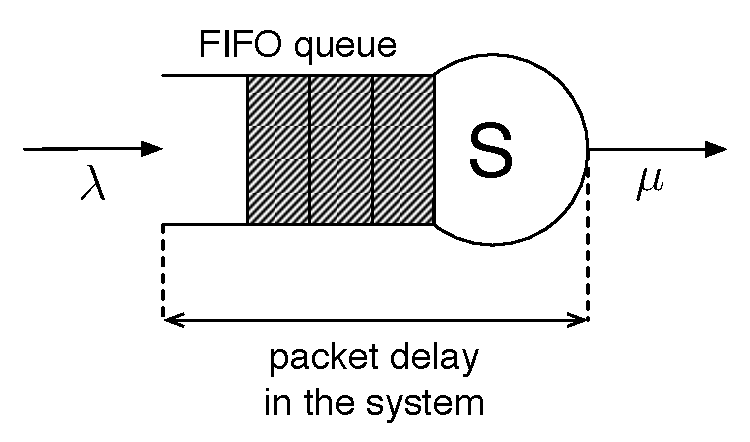
\includegraphics[width=3in]{3/Figures/mm1_queue}
	\caption{Illustration of M/M/1 queuing model}
	\label{fig:mm1_queue_dynamic}
\end{figure}

As a quick reminder of basic queueing theory, M/M/1 queue denotes a single-server queueing system with exponential interarrival times and service times, and a FIFO queue discipline. For a proper, more in-depth treatment of queueing theory, see for example~\cite{CassandrasLafortune2008}. Let $\lambda\in\mathbb{Z}_+$ denote the mean interarrival rate, and let $\mu\in\mathbb{Z}_+$ denote the mean service rate such that $0 \le \lambda < \mu$. The steady-state mean packet delay in an M/M/1 queueing system can thus be defined as follows
\begin{equation}
	\label{eq:mm1_mean_packet_delay_dynamic}
	T = \frac{1}{\mu - \lambda},\quad T\in\displaystyle\left[\frac{1}{\mu}, \infty\right).
\end{equation}
Let $\rho = \displaystyle\frac{\lambda}{\mu}$ denote the mean link (or system) utilization. Clearly, $\rho\in [0,1)$. Hence, the steady-state mean packet delay in Equation~\eqref{eq:mm1_mean_packet_delay_dynamic} can be rewritten as
\begin{equation}
	\label{eq:mm1_mean_packet_delay_2_dynamic}
	T(\rho) = \frac{1}{\mu(1 - \rho)}.
\end{equation}

\begin{table}[p!]
	\caption{Simulation estimated M/M/1 queue steady-state average packet delay}
	\begin{tabular*}{0.5\columnwidth}[L]{@{\extracolsep{\fill}}c c c}
		\hlx{vhv}
		\textbf{Average} & \multicolumn{2}{c}{\textbf{Average packet delay, s}} \\
		\textbf{link utilization} & Mean & $95\%$ confidence interval (x $10^{-5}$) \\
		\hlx{vhv}
		 $0.1$	& $0.02224$	& $4.38835$\\
		 $0.2$	& $0.02497$	& $3.88310$\\
		 $0.3$	& $0.02858$	& $4.32400$\\
		 $0.4$	& $0.03333$	& $6.22518$\\
		 $0.5$	& $0.03999$	& $7.67952$\\
		 $0.6$	& $0.04997$	& $13.62042$\\
		 $0.7$	& $0.06654$	& $22.25786$\\
		 $0.8$	&	$0.10025$	& $51.73063$\\
		 $0.9$	& $0.20100$	& $192.24667$\\
		 \hlx{vhs}
	\end{tabular*}
	\label{tab:mm1_simulation_results_dynamic}
\end{table}
\begin{figure}[p!]
	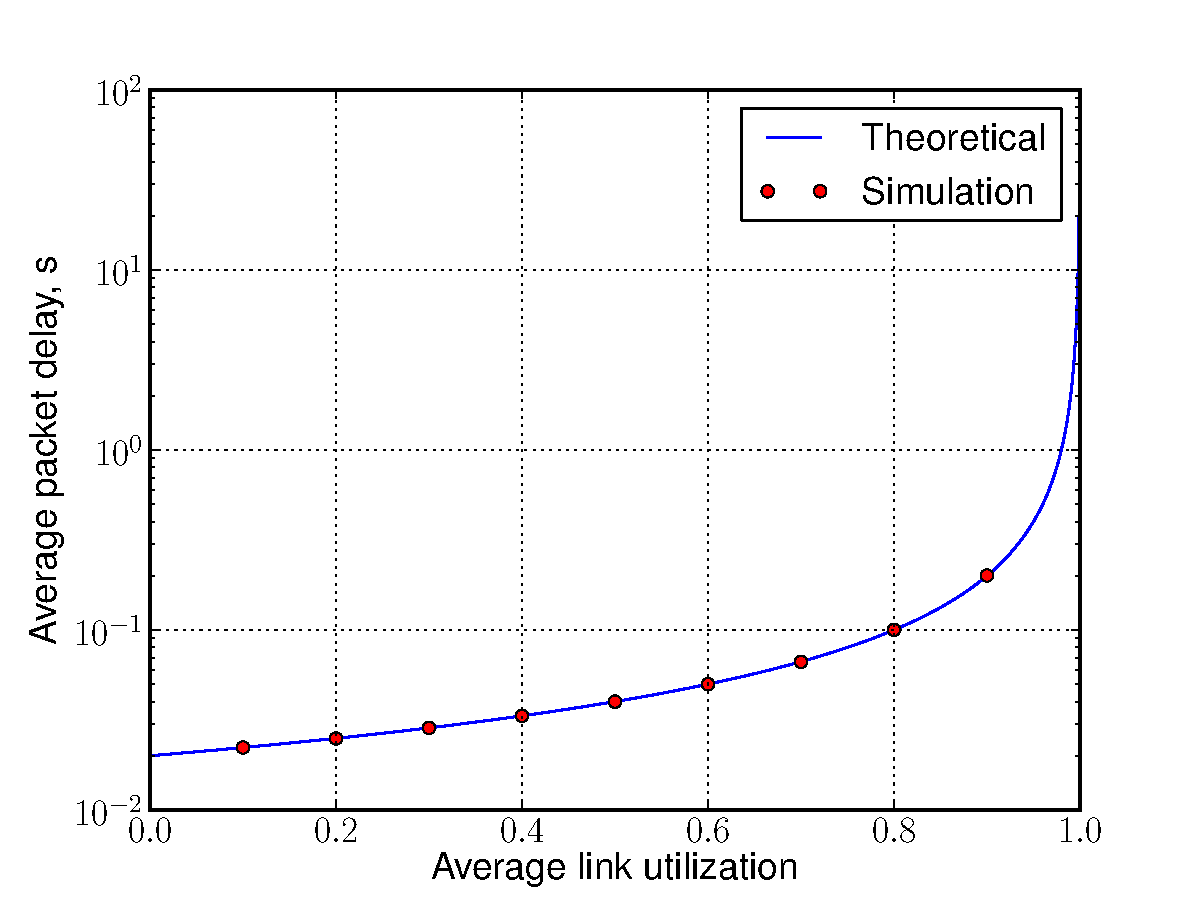
\includegraphics[width=\figsize]{3/Figures/mm1_simulation_results}
	\caption{Comparison of M/M/1 queue simulation results with the theory}
	\label{fig:mm1_simulation_results_dynamic}
\end{figure}

The queueing system was simulated with the following parameters: $\mu=50$ packets per second (pps), and $\lambda\in\{5,10,\ldots,45\}$ pps which is equivalent to $\rho\in\{0.1,0.2,\ldots,0.9\}$. The objective of the simulation was to estimate the steady-state mean packet delay, $T(\rho)$, for each value of the mean link utilization, $\rho$. To this end, for each value of $\rho$, the system was simulated for 1 hour, and a simulation run was replicated 100 times with different seeds to the pseudo-random number generator (PRNG). In all simulation runs, the buffer was initially empty; i.e., there were no packets in the queue. The output of each simulation run constituted a time-series of packet delays in the system. Since the simulation is inherently a nonterminating simulation, the estimation of the steady-state mean packet delay consisted of two steps: 1)~removal of the transient (or warm-up) response of the system, and 2)~averaging within and across the replications with transient response removed. The removal of the transient response was facilitated through the use of the Welch's method~\cite{LawChapter92007}, and for each value of $\rho$, the transient response covered approximately the initial 2000 packet delay samples.

Table~\ref{tab:mm1_simulation_results_dynamic} depicts the estimated steady-state average packet delay for each value of the average link utilization, $\rho$. In all cases, the mean value of the average packet delay closely converges to the theoretical prediction; this conclusion is emphasized in Figure~\ref{fig:mm1_simulation_results_dynamic}. Furthermore, the 95\% confidence interval for the mean of average packet delay does not exceed the factor of $10^{-3}$ for any value of the average link utilization. All in all, this successfully validates the DES simulation engine.
% subsection validation_of_des_simulation_engine (end)

\subsection{Simulation Model of the Digital Marketplace} % (fold)
\label{sub:simulation_model_of_the_digital_marketplace_dynamic}

\subsubsection{High-level Overview} % (fold)
\label{ssub:high_level_overview_dynamic}
The DMP is modeled using the object-oriented paradigm. The entities involved in the DMP are represented by Bidder and DMEventHandler classes. The Bidder class stores attributes specific to a network operator such as costs per service type. The DMEventHandler class, on the other hand, generates subscribers and service requests, runs auctions, etc. Both classes are described in more detail in the next two sections.

When the simulation is running, two types of events are generated: \lstinline{SR_EVENT} and \lstinline{ST_EVENT} (Figure~\ref{fig:dm_events_dynamic}). \lstinline{SR_EVENT} signifies a new service request by a subscriber, and triggers an auction between the network operators; \lstinline{ST_EVENT} signifies that a subscriber has finished using a wireless service, and the servicing network operator can recover any resources dedicated to that subscriber, such as the bit-rate required by the service.
\begin{figure}[t]
	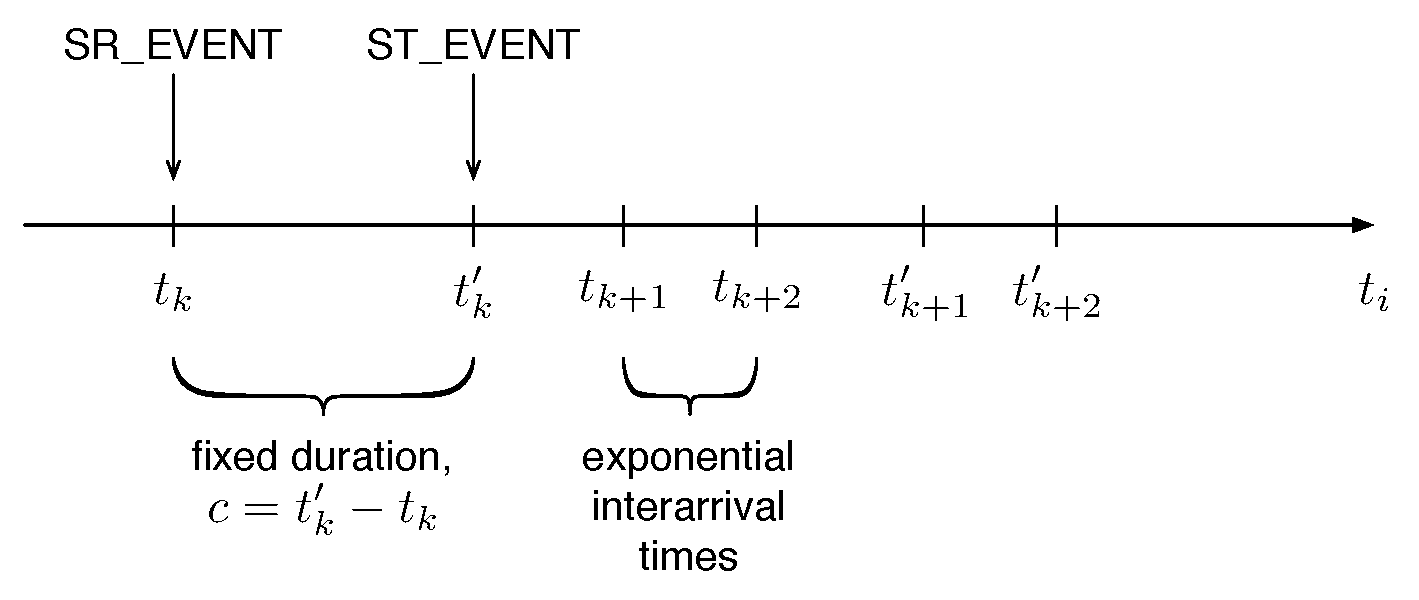
\includegraphics[width=\figsize]{3/Figures/dm_events}
	\caption{Events generated during the simulation of the DMP}
	\label{fig:dm_events_dynamic}
\end{figure}
If we let $t_k$ for all $k\in I$ denote the arrival time of service request $s_k$, then $t_k$ corresponds to the arrival time of an \lstinline{SR_EVENT}. Furthermore, every \lstinline{SR_EVENT} has a corresponding \lstinline{ST_EVENT} such that the time difference between the two is constant; that is, if the arrival time of \lstinline{ST_EVENT} is $t_k'$, then $c = t_k - t_k'$ for all $k\in I$. The time difference $c$ represents the duration of a wireless service requested by a subscriber, and currently, it is assumed to be $c=2.5$ minutes. The interarrival rate of \lstinline{SR_EVENT}s, on the other hand, is currently assumed to be exponentially distributed with parameter $\lambda=1$ service request per second. Since it is difficult to quantify the distribution of the duration of wireless services, it is assumed that the duration is constant in order to keep the model as simple as possible, while, at the same time, the minimum amount of stochasticity is achieved through the exponentially drawn interarrival times of service requests.

In the course of the simulation, the following performance measures are gathered for analysis:
\begin{itemize}
	\item the reputation rating history for each network operator---an indicator of the credibility of network operators over time.
	\item the number of secured auctions (or service requests) by each network operator---an indicator of the market share between network operators over time.
\end{itemize}

It is further assumed that there are two network operators competing in the DMP. This allows for the use of the equilibrium bidding strategy functions derived in Chapter~\ref{cha:network_selection_mechanism_in_the_digital_marketplace}. The subscribers (and  hence, the price weights and service types) are pseudo-randomly generated.
% subsubsection high_level_overview (end)

\subsubsection{Bidder Class} % (fold)
\label{ssub:bidder_class_dynamic}
As mentioned in the High-level Overview section, the Bidder class is tasked with the representation of a network operator. It implements attributes such as costs, current reputation rating, total bit-rate, currently available bit-rate, and subscriber success report list (Figure~\ref{fig:bidder_class_dynamic}). The class also implements the bidding behavior of a network operator, and reputation rating update algorithm. Furthermore, the Bidder class populates subscriber success report list, and updates the currently available bit-rate of a network operator.

\begin{figure}[t]
	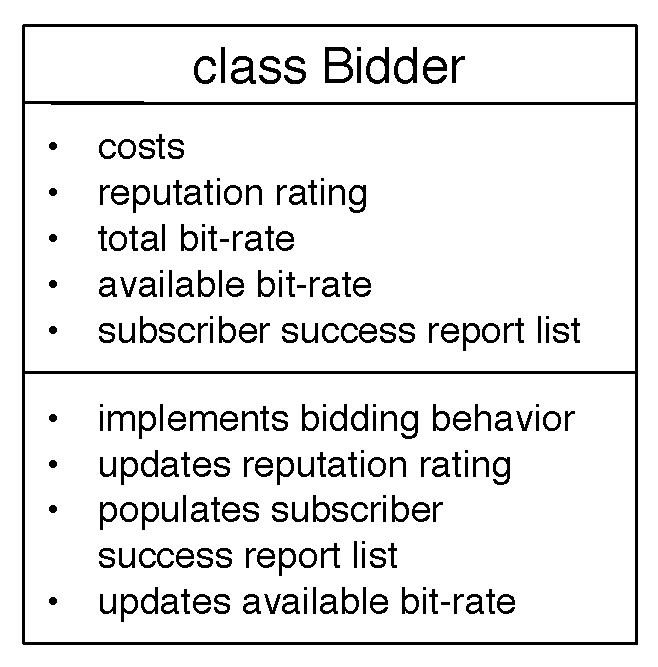
\includegraphics[width=2in]{3/Figures/bidder_class}
	\caption{Bidder class}
	\label{fig:bidder_class_dynamic}
\end{figure}

It is assumed that costs do not change over time, but differ only per service type. Therefore, the cost of web-browsing service might be different from an e-mail service, but neither will change in the course of the simulation. Furthermore, the costs per service type may be specified manually before the simulation executes, or pseudo-randomly drawn from a uniform distribution over the discretized interval $[0,1]$ by the simulation software otherwise.

Initially, the reputation rating is set to $0.5$ for all network operators as discussed in Section~\ref{sec:mathematical_description_dynamic}. Afterwards, for each secured service request by a network operator, the reputation rating is updated according to Equation~\eqref{eq:def_rep_update_lebodic_dynamic}. If a network operator does not secure a service request, then their reputation rating remains constant at that instance of time. For example, if network operator $j$ does not secure a service request at time $t_k$, then $r^j_k = r^j_{k-1}$.

The total available bit-rate has to be manually specified before each simulation for all network operators. The currently available bit-rate, on the other hand, is updated automatically as the simulation progresses. Initially, it equals the total available bit-rate. Then, as a network operator secures service requests, it is decreased by an amount equal to the required bit-rate of the service request for the duration of that service; that is, if network operator $j$ secures service request $s_k$ at time $t_k$, then for $c=2.5$ minutes and provided $t_{k+1}-t_k\le c$, their available bit-rate becomes
\begin{equation*}
	z^j_{k+1} =
	\left\{
	\begin{array}{ll}
		z^j_k - s^{bw}_k &\text{if } z^j_k - s^{bw}_k\ge 0, \\
		0 &\text{otherwise}.
	\end{array}
	\right.
\end{equation*}

The subscriber success report list is updated automatically as the simulation progresses according to Equation~\eqref{eq:def_users_satisfaction_bandwidth_dynamic}. Therefore, if the available bit-rate of the network operator exceeds the required bit-rate of the service, the subscriber is satisfied, and $\sigma_k^j = 1$ is stored in the subscriber success report list. Otherwise, $\sigma_k^j = 0$ is stored.

The Bidder class, by default, assumes that network operators bid myopically; that is, they treat each auction as a one-shot event, and hence, they neglect past as well as future interactions with the other network operators. Although in reality they are likely to bid in a more sophisticated fashion, it is a valid starting point especially in the case of two competing network operators since the analytical solution to a problem of two competing network operators in a one-shot DMP auction exists (see Section~\ref{sec:indirect_approach_static}, Chapter~\ref{cha:network_selection_mechanism_in_the_digital_marketplace}). 

The Bidder and the DMEventHandler classes interface according to the following sequence:
\begin{enumerate}
	\item \lstinline{SR_EVENT} (and hence, service request with all the relevant parameters) is generated;
	\item DMEventHandler class calls for an auction;
	\item an object of Bidder type (and hence, network operators) submit their bids according to the implemented bidding behavior;
	\item DMEventHandler class elects the winner of the auction;
	\item \lstinline{ST_EVENT} is generated for the winner;
	\item reputation rating, available bit-rate, and subscriber success report list are updated accordingly.
\end{enumerate}
% subsubsection bidder_class (end)

\subsubsection{DMEventHandler Class} % (fold)
\label{ssub:dmeventhandler_class_dynamic}
\lstinline{SR_EVENT} exponential interarrival times; \lstinline{ST_EVENT} is scheduled after each \lstinline{SR_EVENT} at a constant interval of 2.5 minutes. Stores possible service request types such as \lstinline{WEB_BROWSING} and \lstinline{EMAIL} with their required bit-rates. Currently, it is assumed that \lstinline{WEB_BROWSING} requires 512 kbps, while \lstinline{EMAIL} requires 256 kbps. DMEventHandler also runs auctions and elects the winner. FIX:ME

\begin{figure}[t]
	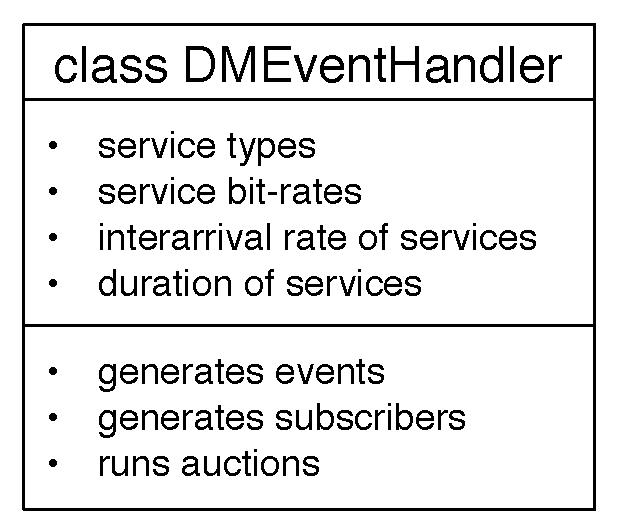
\includegraphics[width=2in]{3/Figures/dmeventhandler_class}
	\caption{DMEventHandler class}
	\label{fig:dmeventhandler_class_dynamic}
\end{figure}
% subsubsection dmeventhandler_class (end)

% subsection simulation_model_of_the_digital_marketplace (end)
% section simulation_modeling (end)

\section{Simulation Scenarios and Analysis} % (fold)
\label{sec:simulation_scenarios_and_analysis_dynamic}
Analyze reputation rating update systems proposed by Alisdair and Le Bodic. Compare and contrast. Show that they are initial conditions sensitive.
% section simulation_scenarios_and_analysis (end)

\section{Summary} % (fold)
\label{sec:summary_dynamic}

% section summary (end)

% chapter dynamics_of_network_selection_in_the_digital_marketplace (end)
